\newpage
\section{Durchführung und Aufbau}
\label{sec:Durchführung}
\subsection{Aufbau}
In Abbildung (\ref{fig:aufbau}) ist der Aufbau des Versuches dargestellt.
\begin{figure}
	\centering
	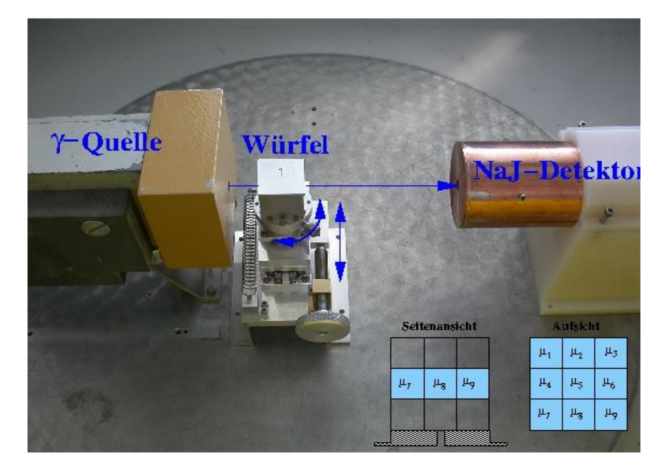
\includegraphics[scale=0.5]{fig/aufbau.png}
	\caption{Versuchaufbau bestehend aus Szintillator, $\gamma$-Quelle und Plattform für die Würfel \cite[2]{Anleitung}.}
	\label{fig:aufbau}
\end{figure}
\FloatBarrier
\noindent Wie in Abbildung (\ref{fig:aufbau}) zu sehen wird die mittlere Schicht des jeweiligen Würfels untersucht. Diese besteht wiederum aus neun Elementarwürfeln. Die Strahlungsquelle
ist mit Bleiblöcken abgeschirmt und mit einer Bleiblende wird die Strahlung auf den Würfel bzw. den Detektor fokussiert. Zusätzlich schützen die Bleiblöcke den Experimentierenden vor Strahlung. In den Strahlengang zwischen $\gamma$-Quelle und Szintillator befindet sich ein Podest, welches zur Justierung
der Würfel für die verschiedenen Projektionen verwendet wird.\\
Szintillator und Photomultiplier (PM) dienen zusammen als Detektor. Im Gegensatz zu einem organischen Szintillator, der sich durch seine gute Zeitauflösung auszeichnet, wird in diesem Versuch ein anorganischer Szintillator verwendet, der eine wesentlich bessere Energieauflösung
besitzt. Die $\gamma$-Strahlung dringt in den Szintillator ein und regt Elektronen an, welche dann Aktivator-Zentren innerhalb des verwendeten Kristalls anregen. Nachdem diese angeregt
wurden, fallen sie unter Aussendung eines Photons wieder in den Grundzustand zurück. Das dadurch entstandende Licht wird nun wiederum vom PM in ein elektrisches Signal umgewandelt. Die
Amplitude dieses Signals ist proportional zur Energie des Lichts und wird mit einem Multichannel Analyzer (MCA) histogrammiert. Am Computer, der ebenfalls zum Aufbau des Versuches gehört, kann die Messung graphisch ausgelesen werden.
\subsection{Durchführung}
Als erstes wird zur Bestimmung der Intensität $I_\mathrm{0}$ die leere Aluminiumhülle in den Strahlengang gestellt und ein Spektrum wird aufgenommen, dabei wird die Projektion 2
verwendet (siehe Zeile 2 der Geometriematrix in Gleichung (\ref{eqn:geomat})). Es werden die Würfel, die nur aus Aluminium bzw. nur aus Blei bestehen, vermessen. Dabei werden vier
Messungen vorgenommen, die jeweils eine andere Weglänge haben. Als letztes wird nun der Würfel aus unbekanntem Material vermessen, hier müssen im Gegensatz zu den anderen Würfeln
zwölf Messungen durchgeführt werden. Dabei werden nacheinander die Projektionen aus der Geometriematrix in Gleichung (\ref{eqn:geomat}) verwendet.
